	\newcommand{\figscale}{0.6}
\chapter{Content Tracking}
\minitoc

Our change tracking system relies on a version control system underneath that provides us with a database of the history of how each tracked file changes.  We choose the content tracking system called ``git,'' \cite{git} as it matches with important requirements of our system:
\begin{itemize}
\item distributed usage: authors maintain their own repository and efficiently share and merge others, as well as superior offline capabilities
\item available on major platforms %check about Windows!
\item free and open source
\end{itemize}

\section{Traversing History}

\begin{figure}
\centering
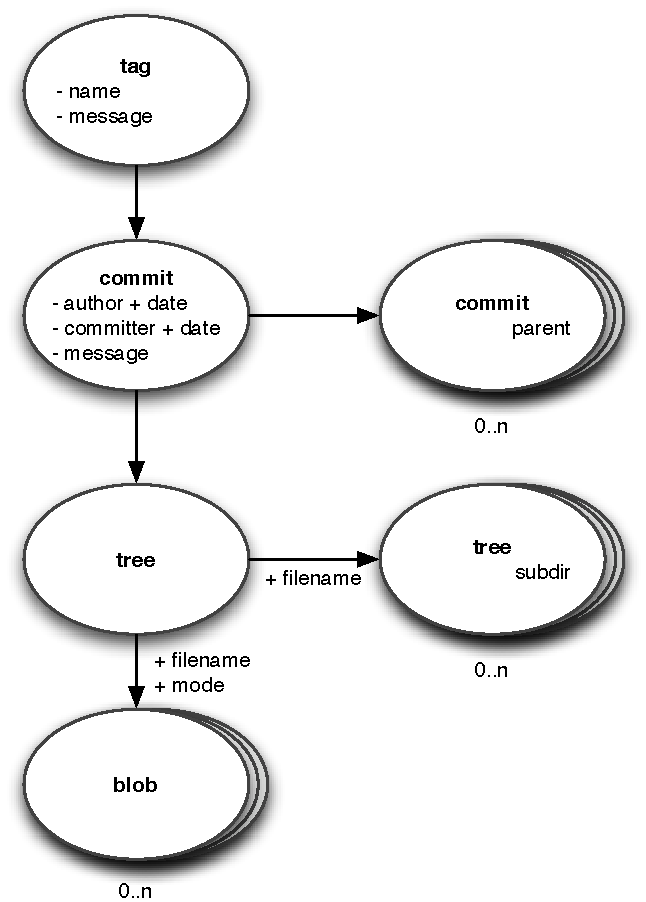
\includegraphics[scale=\figscale]{./figures/git-nodes}
\caption{Node types in Git repositories} \label{fig:git-nodes}
\end{figure}
The anatomy of a git repository is a \textit{directed, acyclic graph} (DAG) with various pointers maintained. There are four types of nodes, which are immutable objects denoted by an SHA-1 hash.  See Figure~\ref{fig:git-nodes} for a graphical representation. 
\begin{enumerate}
\item blob: A leaf node that is the simplest object in git.  Most often it represents a file but can also refer to symbolic links and other artifacts.
\item tree: A tree node encapsulate a directory in git.  It points to blobs and other trees that are subdirectories of this directory.
\item commit: A commit node refers to one tree that represents the state of the files at the time of the commit.  It also refers to other commit nodes that are its parents.  An initial commit has no parents.  A merged commit has more than one parent.
\item tag: A tag node points to one commit.
\end{enumerate}

To obtain the history of a single file in git, we have to traverse the DAG of the commits (more precisely, the tree rooted at the head commit of the currently checked out branch) and search for this individual file in the subtree under each commit.  Figure~\ref{fig:git-commit1} shows an example where a file \texttt{foo.tex} has been modified in a few commits and most notably in the parallel branches.

\begin{figure}
\centering
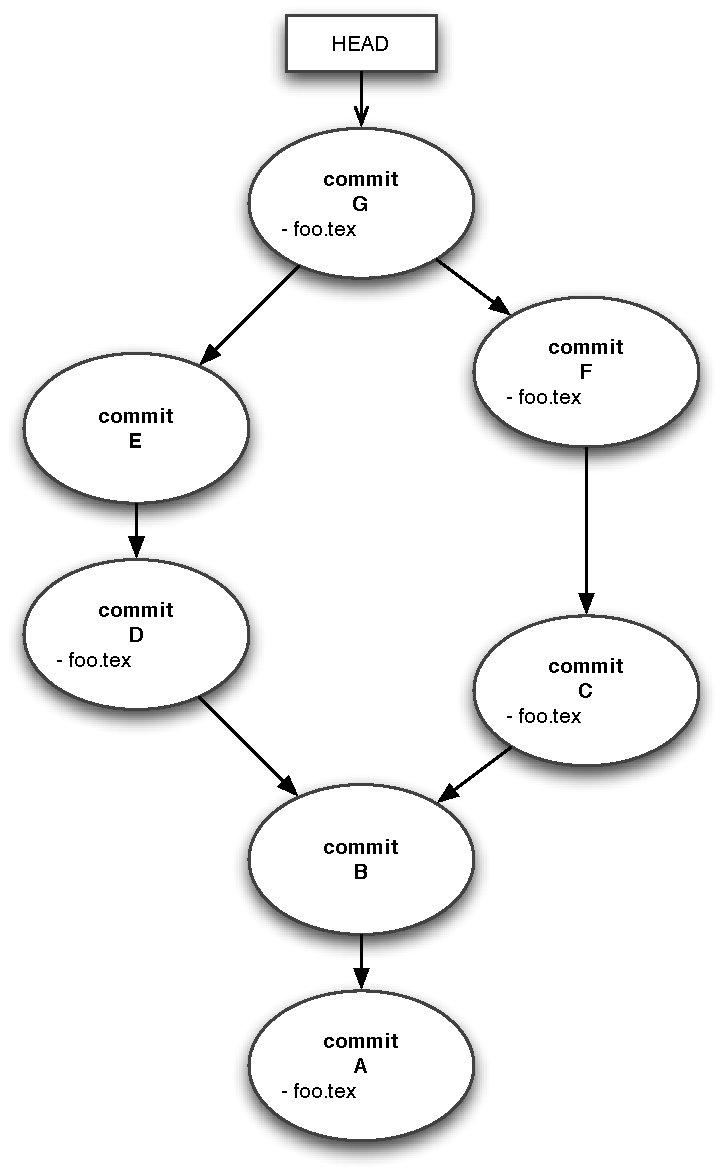
\includegraphics[scale=\figscale]{./figures/git-commit-history1}
\caption{Example commit history for certain file \texttt{foo.tex}} \label{fig:git-commit1}
\end{figure}

As git provides many tools and scripts to deal with the repository, we suggest a two step approach:  First, we obtain the log of the file to identify the commits, in which the contents of the file changed.  Then, we create specialized diffs between each pair of file versions that are adjacent in the history of that file.  Note that the history of the file can be non-linear when branches contain parallel modifications of the file.

\subsection{Commit Graphs}

Here we introduce a few mathematical definitions to be used to clarify the specification of how the change history of a given file is computed.  We assume that the file in question is tracked in a git repository\footnote{We further assume that the git repository currently does not have a detached HEAD reference.}.

\begin{defi}[Commit Graph]
The commit graph $G \subset N \times N$, where $N$ is the set of commit nodes in git, is obtained from traversing the history of commits starting from the HEAD reference until no more nodes can be reached.  The commit graph is directed and acyclic. 
\end{defi}

Most likely, the user's current filter on viewing changes contains a date or revision identifier that will be used to prune the commit graph.

\begin{defi}[Time-Pruned Commit Graph]
We obtain the time-pruned commit graph for a given date as follows.  Traverse the commit graph from the HEAD in a modified breadth-first search (in that nodes can be visited more than once and the resulting graph is not necessarily a tree).  When the given date is later than a commit encountered from traversing the graph, the node is not included in the pruned graph and the search continues at the parent.  Then, all nodes in the resulting graph have time stamps that are later or at the given date.
When the graph is pruned by revision identifier, we follow the same procedure as above with the time stamp of the commit node denoted by the revision identifier.
\end{defi}

\begin{figure}
\centering
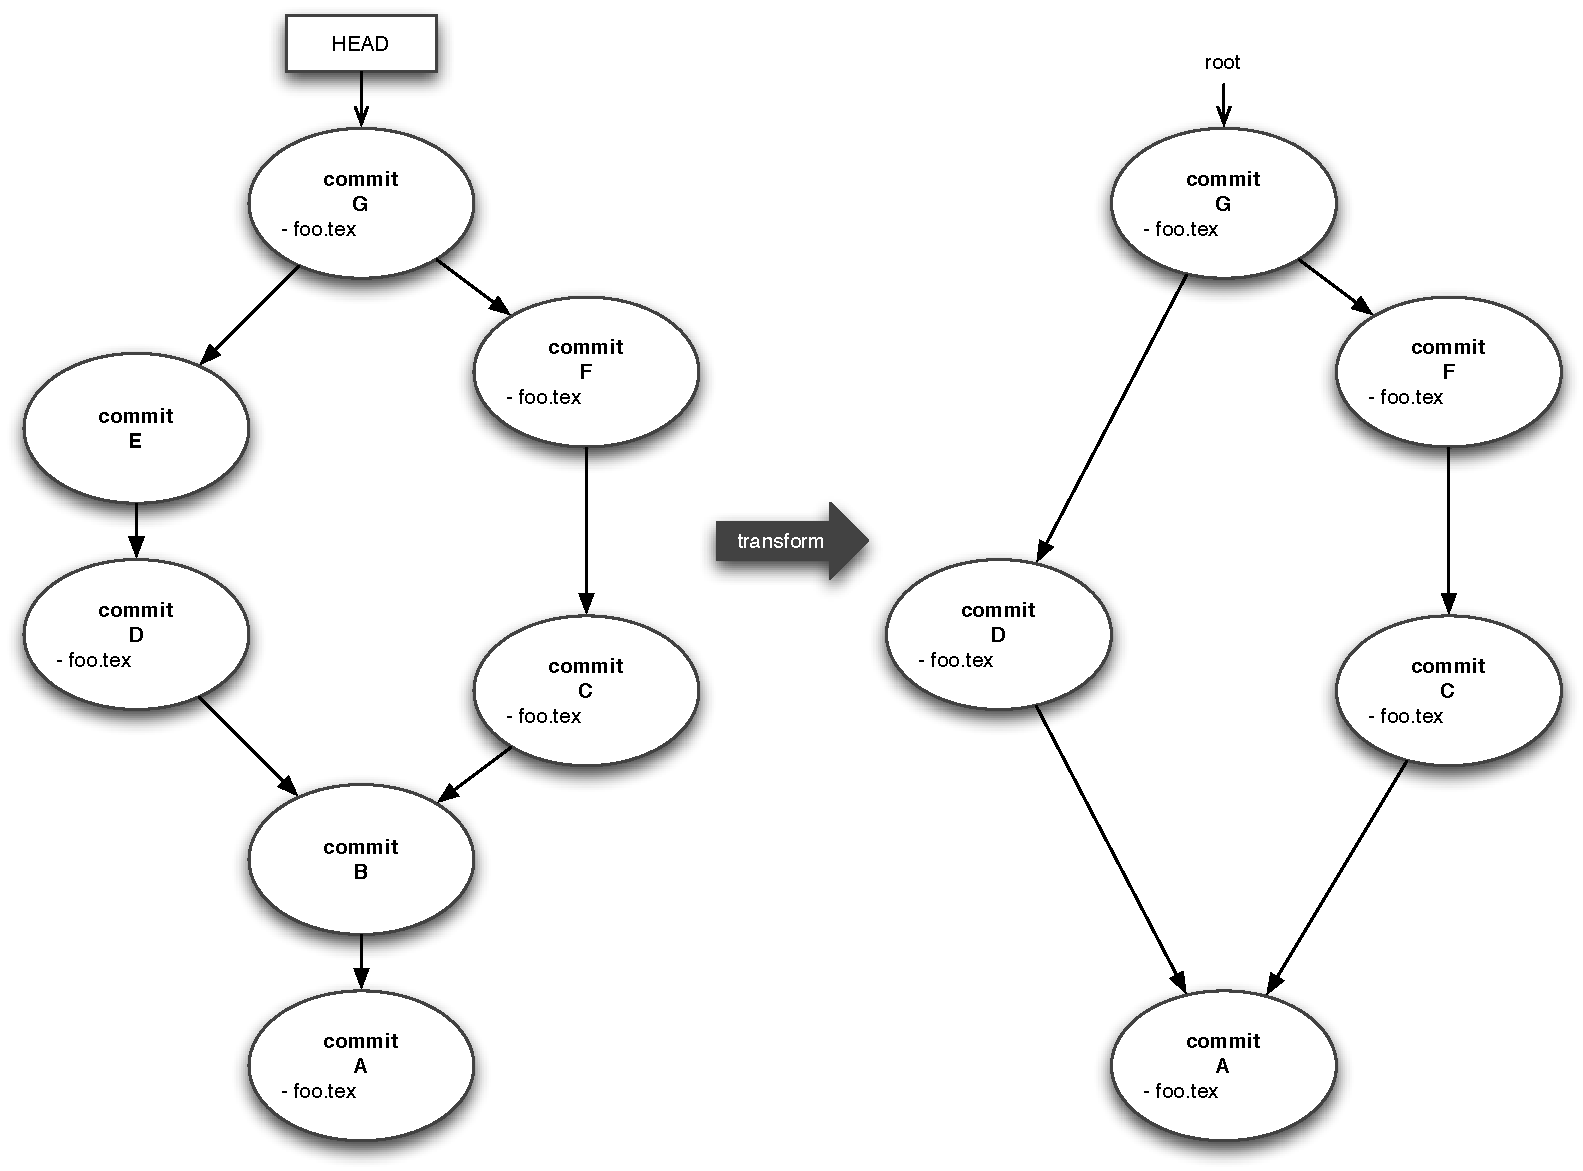
\includegraphics[width=0.9\textwidth]{./figures/git-commit-history2b}
\caption{Transforming commit graph given file \texttt{foo.tex}} \label{fig:git-commit2b}
\end{figure}

Next, we describe how to transform the (potentially time-pruned) commit graph when we obtain the changes of a certain file.  Figure~\ref{fig:git-commit2b} depicts an example of this transformation.

\begin{defi}[File-Specific Commit Graph]
We mark all commit nodes that contain changes to the given file as the set $N^{*} \subseteq N$. Then, we traverse the commit graph again from the HEAD pointer, this time in depth-first search (with the modification of visiting nodes multiple times, as the resulting graph is not necessarily a tree). If the visited node $n_{current}$ is element of $N^{*}$, we include it in the new graph. Keeping track of the last node added (or, if this is the first one, we use the HEAD reference), we add the edge $(n_{last\_added}, n_{current})$ to the new, file-specific commit graph $G^{*}$. If $n_{current}$ is already part of the graph, we backtrack to the next branch to traverse.  When backtracking, the pointer to the last node added has to be adjusted.
\end{defi}

\begin{lem}
The transformed file-specific commit graph is always rooted at exactly one commit node.  If during traversal we encounter a merge commit node with more than one child, and at least two branches under this parent contain changes to the given file, then the merge commit must also contain changes to the said file and thus have the merge commit be included in $G^{*}$.  Therefore, we cannot construct a situation, in which the root pointer would reference more than one commit node in $G^{*}$.
\end{lem}

\begin{figure}
\centering
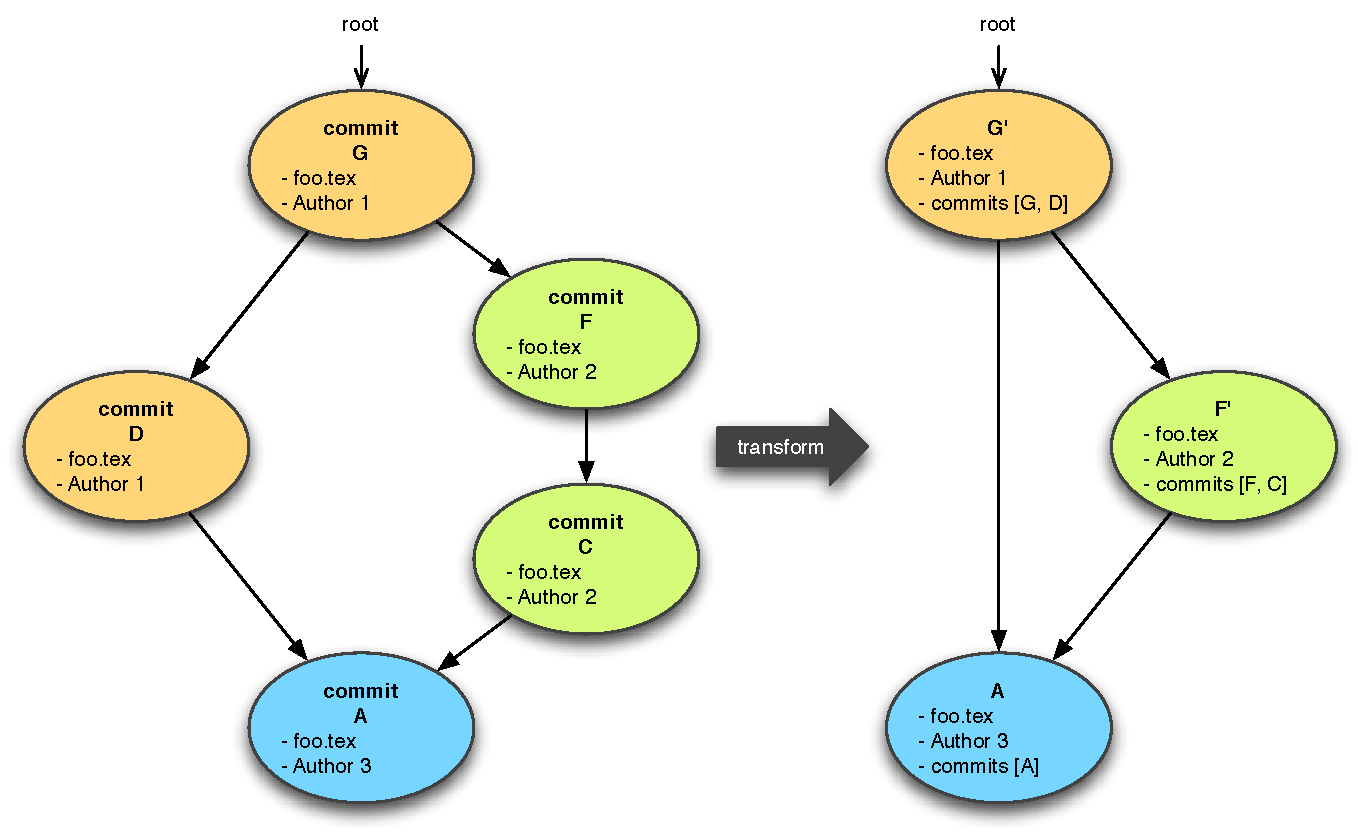
\includegraphics[width=0.9\textwidth]{./figures/git-commit-history3b}
\caption{Subsuming commits of same authors} \label{fig:git-commit3b}
\end{figure}

Finally, we describe how the new commit graph gets further transformed to subsume subsequent edits of the same author. Figure~\ref{fig:git-commit3b} shows such an example transformation.  We decide to only subsume subsequent commits if they are part of a linear commit history in the commit graph.  When the date, time, and revision information of subsumed commits is displayed to the user, there will be ranges as a subsumed commit node now potentially refers to multiple commits from the original graph.

more details and definitions for collapsing commits by same author
%\begin{defi}[Author-Subsumed Commit Graph]
%We traverse a given commit graph again using (a modified) depth-first search.  We take note of the author name in the last commit node visited $s_{last\_author}$.  If the currently visited node has the same author name, we build up a list of references to the original commit node and drop this node
%\end{defi}

%\begin{figure}
%\centering
%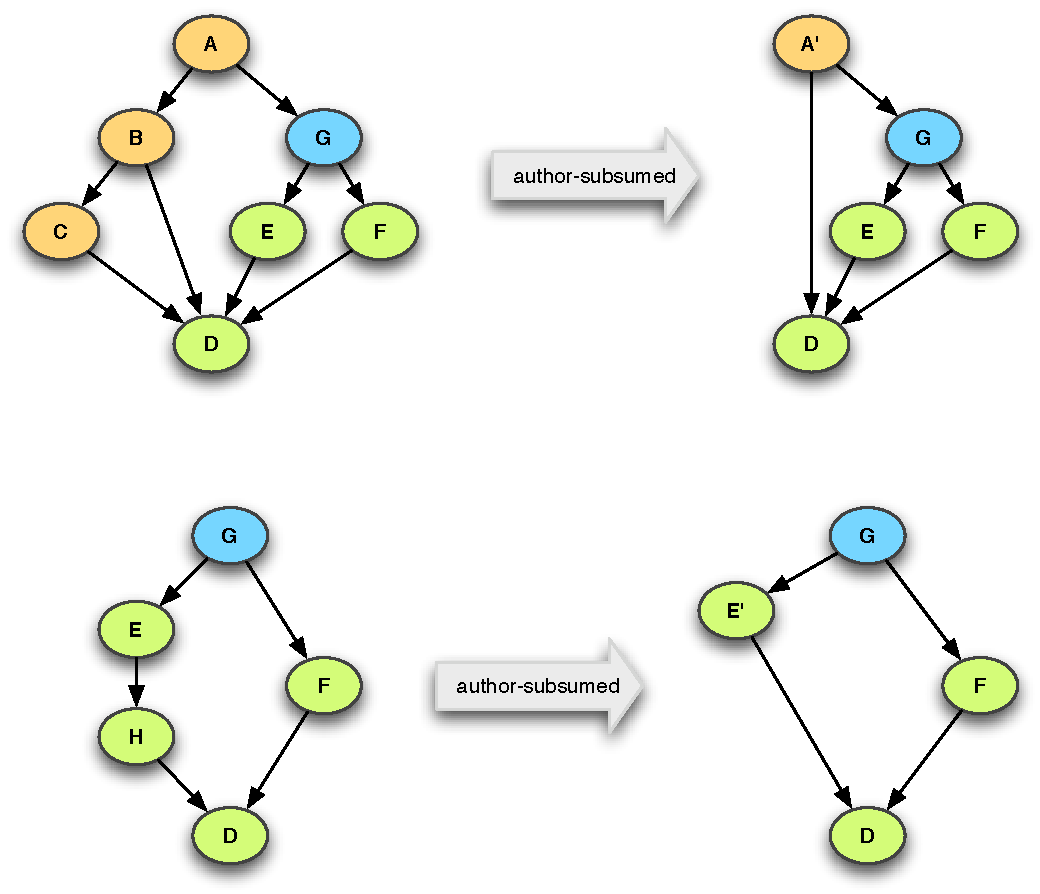
\includegraphics[width=0.9\textwidth]{./figures/tmp-examples}
%\caption{2 examples to discuss} \label{fig:tmp-examples}
%\end{figure}

%Subsume adjacent commits by same author under the latest one?  Makes sense when looking at many commits (we might commit automatically every time the editing author saves when in LTC mode). Also makes sense as LTC is motivated by being interested in other people's changes but not how often or fine-grained the author's commits are.

\section{Serializing Parallel Changes}

%\begin{figure}
%\centering
%%
%\caption{Example of serializing parallel branches for accumulating changes} \label{fig:example-serialization}
%\end{figure}

If we encounter branches in the commit graph, we serialize the parallel changes using the date and time information in the last commit node before the merge commit.  Then, the changes are applied in order of the time stamps.%, as Figure~\ref{fig:example-serialization} depicts.




\section{Filtering}

Filtering the view of changes is the central element to provide real usability of our change tracking capability.  Table~\ref{tab:filter} gives an overview of the choices the user can make to filter the amount of changes displayed.

\begin{table}
\centering
\begin{tabular}{cp{3.5in}p{1.1in}} \toprule
& Description & Default \\\midrule
Authors & If a set of author names is given, limit the view of changes to only those that the respective authors made. To view own changes, include editing author in set. & empty \\
Date/Revision & Specify a time or revisions of how far back to view.  By default, the view extends back to the last commit of the editing author that was before any commit of another author. & last commit until now\\
``Small Changes'' & choose to view changes in words of length $\geq 3$ and Levenshtein distance between words $\leq 3$ & suppress changes \\
%White Space & choose to view changes in white space (unless it affects LaTeX output such as $\geq 2$ consecutive newlines that create a paragraph) & suppress changes \\
Deletions & choose to view deletions & view changes \\
LaTeX Preamble & choose to view changes in LaTeX preamble & view changes \\
LaTeX Markup & choose to view changes in LaTeX markup (commands) & view changes \\
LaTeX Comments & choose to view changes in LaTeX comments & suppress changes \\
\bottomrule
\end{tabular}
\caption{Filtering options} \label{tab:filter}
\end{table}

more details